% !TeX root = surprises.tex

\chapter{Resolución de ecuaciones cuadráticas}\label{c.quadratic}

%%%%%%%%%%%%%%%%%%%%%%%%%%%%%%%%%%%%%%%%%%%%%%%%%%%%%%%%%%%%%%%

Poh-Shen Loh propuso un método para resolver ecuaciones cuadráticas que se basa en una relación entre los coeficientes del polinomio cuadrático y sus raíces. Sección~\ref{s.traditional} revisa los métodos tradicionales para resolver ecuaciones cuadráticas. 
La sección~\ref{s.computing} intenta convencer al lector de que el método de Loh tiene sentido y luego explica cómo calcular las raíces. En la sección ~\ref{s.examples} se realiza el cálculo para dos polinomios cuadráticos y un cálculo similar para un polinomio cuártico. La sección~\ref{s.general} deriva la fórmula tradicional para las raíces a partir de las fórmulas de Loh.

La introducción del álgebra y de la notación algebraica moderna es relativamente reciente. Anteriormente, los matemáticos utilizaban la geometría casi exclusivamente, por lo que es interesante observar la construcción geométrica de al-Khwarizmi de la fórmula para las raíces de ecuaciones cuadráticas (Sec.~\ref{s.khwar}). La sección~\ref{s.cardano} muestra una ingeniosa construcción geométrica utilizada por Cardano en el desarrollo de la fórmula para las raíces de ecuaciones cúbicas.

La sección~\ref{s.lill-quadratic} presenta otros métodos geométricos para hallar las raíces de ecuaciones cuadráticas\footnote{El capítulo~\ref{c.origami-cube} es un prerrequisito para una comprensión completa de estos métodos.}. El capítulo concluye con la sección~\ref{s.numerical}, que trata del cálculo numérico de las raíces de ecuaciones cuadráticas.

\section{Métodos tradicionales para resolver ecuaciones cuadráticas}\label{s.traditional}
\index{Quadratic equation}
Todo estudiante de matemáticas memoriza la fórmula para obtener las raíces de una ecuación cuadrática $ax^2+bx+c=0$:
\[
x_1, x_2 = \frac{-b\pm\sqrt{b^2-4ac}}{2a}\,.
\]                      
Por ahora trabajaremos con polinomios mónicos, $x^2+bx+c=0$, cuyas raíces son:
\begin{align}
x_1, x_2 = \frac{-b\pm\sqrt{b^2-4c}}{2}\,.\label{eq.quadratic-roots}
\end{align}
Otro método para resolver ecuaciones cuadráticas consiste en factorizar los polinomios más o menos por ensayo y error. A veces es fácil obtener las raíces mediante factorización:
\begin{align}
x^2-4x+3= (x-1)(x-3)\label{eq.quadratic-lill}\,.
\end{align}
Es mucho más difícil factorizar $x^2-2x-24$ porque hay muchos pares posibles de raíces que hay que considerar:
\[
(\pm 1,\mp 24)\,, (\pm 2,\mp 12)\,, (\pm 3,\mp 8)\,, (\pm 4,\mp 6)\,.
\]

\vspace*{-3ex}

\section{La relación entre las raíces y los coeficientes}\label{s.computing}
\index{Quadratic equation!roots of}

\begin{theorem}\label{thm.roots-coefficients}
Si $r_1,r_2$ son las raíces de $x^2+bx+c$ entonces:
\[
(x-r_1)(x-r_2)=x^2 - (r_1+r_2)x + r_1r_2=x^2+bx+c\,.
\]
Por lo tanto, aunque no conozcamos los valores de las raíces, sí sabemos que:
\begin{align}\label{eq.viete-quad}
r_1+r_2 = -b\,,\quad\quad r_1r_2=c\,.
\end{align}
\end{theorem}
\noindent{}En realidad no hay nada que demostrar porque el resultado surge del cálculo.

\noindent{}Consideremos algunos valores de $-b,r_1,r_2$ y sea $m_{12}$ la media de $r_1,r_2$:
\[
\renewcommand{\arraystretch}{1.2}
\begin{array}{|@{\hspace{1em}}r|@{\hspace{1em}}r|@{\hspace{1em}}r|@{\hspace{1em}}r|}
\hline
-b& r_1 & r_2 &m_{12}\\\hline
33 & 12 & 21 & 16\frac{1}{2}\\\hline
33 & 8 & 25 & 16\frac{1}{2}\\\hline
33 & 1 & 32 & 16\frac{1}{2}\\\hline\hline
-b& r_1 & r_2 &m_{12}\\\hline
-4 & -16 & 12 & -2 \\\hline
-4 & -4 & 0 & -2 \\\hline
-4 & -3 & -1 & -2 \\\hline
\end{array}
\]
Para cualquier ecuación cuadrática la media de las dos raíces es constante:
\[
m_{1,2}=\frac{r_1+r_2}{2}=
\frac{(-b-r_2)+r_2}{2}=
-\frac{b}{2}\,.
\]
Sea $s$ un número cualquiera. Entonces:
\[
-b=-b+s+(-s)=\left(\frac{-b}{2}+s\right) + \left(\frac{-b}{2}-s\right)=r_1+r_2\,.
\]
Si una raíz está a distancia $s$ de la media, la otra raíz está a distancia $-s$ de la media. Para $r_1,r_2=2,6$, donde $m_{12}=4, s=2$, tenemos:
\[
\renewcommand{\arraystretch}{1.2}
\begin{array}{|@{\hspace{1em}}r|@{\hspace{1em}}r|@{\hspace{1em}}r|@{\hspace{1em}}r|r|r|}
\hline
-b& r_1 & r_2 & m_{12}& m_{12}\!-\!r_1 & m_{12}\!-\!r_2\\\hline
33 & 12 & 21 & 16\frac{1}{2}&4\frac{1}{2} & -4\frac{1}{2}  \\\hline
33 & 8 & 25 & 16\frac{1}{2}&8\frac{1}{2}&-8\frac{1}{2}\\\hline
33 & 1 & 32 & 16\frac{1}{2}&15\frac{1}{2}&-15\frac{1}{2}\\\hline
\hline
-4 & -16 & 12 & -2 &14& -14\\\hline
-4 & -4 & 0 & -2&2&-2 \\\hline
-4 & -3 & -1 & -2&1&-1 \\\hline
\end{array}
\]
La figura~\ref{f.loh-roots1} visualiza esta relación.
\begin{figure}[t]
\begin{center}
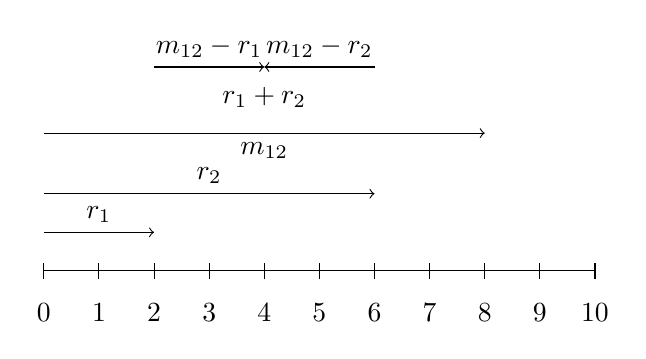
\begin{tikzpicture}[scale=.7]
\begin{scope}[yshift=-4mm]
\draw (0,0) -- (10,0);
\foreach \x in {0,1,...,10}
  \draw (\x,-1.5mm) -- +(0,3mm) node[below,yshift=-4mm] {$\x$};
\draw[->,yshift=7mm] (0,0) -- node[above] {$r_1$} (20mm,0);
\draw[->,yshift=14mm] (0,0) -- node[above] {$r_2$} (60mm,0);
\end{scope}
\draw[->,yshift=21mm] (0,0) -- node[above,yshift=2mm] {$r_1+r_2$} (80mm,0);
\coordinate (M) at (40mm,21mm);
\vertex{M};
\node[below] at (40mm,21mm) {$m_{12}$};
\begin{scope}[yshift=3mm]
\draw[->,yshift=30mm] (20mm,0mm) -- node[above] {$m_{12}-r_1$} +(20mm,0);
\draw[->,yshift=30mm] (60mm,0mm) -- node[above] {$m_{12}-r_2$} +(-20mm,0);
\end{scope}
\end{tikzpicture}
\end{center}
\caption{Relación entre las raíces $r_1,r_2=2,6$ y su media $m_{12}=4$}
\label{f.loh-roots1}
\end{figure}
Si utilizamos otros valores $r_1,r_2=3,5$ para los que $r_1+r_2=8$ entonces $m_{12}=4$ permanece igual mientras que $s$ se convierte en $1$ (Fig.~\ref{f.loh-roots2}).

El desplazamiento $s$ parece ser arbitrario en:
\[
r_1=\left(\frac{-b}{2}+s\right)\,,\quad r_2=\left(\frac{-b}{2}-s\right)\,,
\]
\noindent{}pero hay una restricción adicional $r_1r_2=c$, donde $c$ es el término constante del polinomio.
Multiplicando las dos expresiones que hemos obtenido para $r_1,r_2$, podemos determinar $s$ y luego $r_1,r_2$:
\begin{eqnarray*}
c&=&\left(-\frac{b}{2} +s\right)\left(-\frac{b}{2} -s\right)=
  \frac{b^2}{4}-s^s\\
s&=&\frac{\sqrt{b^2-4c}}{2}\,.
\end{eqnarray*}

\begin{figure}[t]
\begin{center}
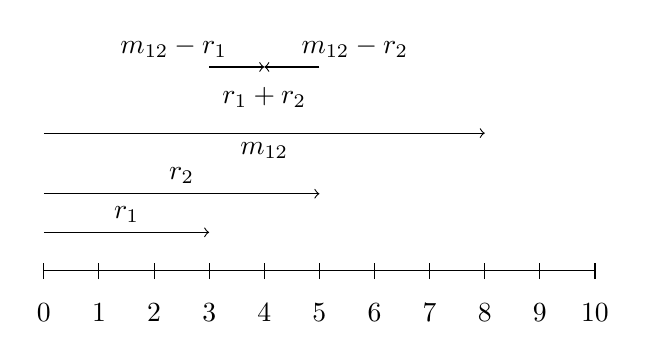
\begin{tikzpicture}[scale=.7]
\begin{scope}[yshift=-4mm]
\draw (0,0) -- (10,0);
\foreach \x in {0,1,...,10}
  \draw (\x,-1.5mm) -- +(0,3mm) node[below,yshift=-4mm] {$\x$};
\draw[->,yshift=7mm] (0,0) -- node[above] {$r_1$} (30mm,0);
\draw[->,yshift=14mm] (0,0) -- node[above] {$r_2$} (50mm,0);
\end{scope}
\draw[->,yshift=21mm] (0,0) -- node[above,yshift=2mm] {$r_1+r_2$}(80mm,0);
\coordinate (M) at (40mm,21mm);
\vertex{M};
\node[below] at (40mm,21mm) {$m_{12}$};
\begin{scope}[yshift=3mm]
\draw[->,yshift=30mm] (30mm,0mm) -- node[above left] {$m_{12}-r_1$} +(10mm,0);
\draw[->,yshift=30mm] (50mm,0mm) -- node[above right] {$m_{12}-r_2$} +(-10mm,0);
\end{scope}
\end{tikzpicture}
\end{center}
\caption{Relación entre las raíces $r_1,r_2=3,5$ y su media $m_{12}=4$}
\label{f.loh-roots2}
\end{figure}

\section{Ejemplos del método de Loh}\label{s.examples}

\begin{example}
Consideremos el polinomio $x^2-2x-24$ donde $b=-2,c=-24$:
\begin{eqnarray*}
c&=&\left(-\frac{(-2)}{2} +s\right)\left(-\frac{(-2)}{2} -s\right)\\
-24&=&(1 +s)(1 -s)\\
%s^2&=&25\\
s&=&5\\
r_1&=&1+5=6\\
r_2&=&1-5=-4\,.
\end{eqnarray*}
Verifiquemos: $(x-6)(x-(-4))= x^2-2x-24$.
\end{example}

\begin{example}
Busquemos las raíces de $x^2-83x-2310$:
\begin{eqnarray*}
%c&=&\left(-\frac{b}{2} +s\right)\left(-\frac{b}{2} -s\right)\\
-2310&=&\left(\frac{83}{2}+s\right)\left(\frac{83}{2} -s\right)\\
s^2&=&\frac{6889}{4}+2310=\frac{16129}{4}\\
s&=&\frac{127}{2}\\
r_1&=&\frac{83}{2}-\frac{127}{2}=-22\\
r_2&=&\frac{83}{2}+\frac{127}{2}=105\,.
\end{eqnarray*}
Verifiquemos: $(x+22)(x-105)= x^2-83x-2310$.

Controlemos este cálculo con el cálculo mediante la fórmula tradicional:
\begin{eqnarray*}
\frac{-b\pm\sqrt{b^2-4c}}{2}&=&\frac{-(-83)\pm\sqrt{(-83)^2-4\cdot (-2310)}}{2}\\
%&=& \frac{83\pm\sqrt{6889+9240}}{2} = \frac{83\pm\sqrt{16129}}{2}\\
&=& \frac{83\pm\sqrt{16129}}{2} = \frac{83\pm 127}{2}\\
r_1&=&\frac{83-127}{2}=-22\\
r_2&=&\frac{83+127}{2}=105\,.
\end{eqnarray*}
\end{example}

\begin{example}
Teorema~\ref{thm.roots-coefficients} puede generalizarse a polinomios de grados superiores. He aquí un ejemplo interesante para una \emph{ecuación cuártica} $x^4-10x^2-x+20=0$. Al igual que con las ecuaciones cuadráticas, existen fórmulas para resolver ecuaciones cúbicas y cuárticas (aunque no ecuaciones de potencias superiores), pero las fórmulas son bastante complicadas.

¿Se podrá factorizar este polinomio de grado cuatro en dos polinomios cuadráticos con coeficientes enteros? Si es así, los coeficientes de los términos $x$ en los factores cuadráticos deben ser \emph{iguales y de signos opuestos} ya que el coeficiente del término $x^3$ en el polinomio cuártico es cero. Por lo tanto, la forma de los factores cuadráticos es:
\[
f(x) = (x^2 - nx + k_1)\, (x^2 + nx + k_2)\,.
\]
Realizando la multiplicación se obtiene:
\[
\renewcommand{\arraystretch}{1.1}
\begin{array}{rrrrrr}
f(x) = &x^4 & + nx^3 & + k_2 x^2\\
&& -nx^3 &- n^2x^2 &-nk_2x\\
&&&+k_1x^2 &+ nk_1x &+ k_1k_2\,.
\end{array}
\]
Igualando los coeficientes se obtienen tres ecuaciones con tres incógnitas $n,k_1,k_2$:
\begin{eqnarray*}
(k_1+k_2)-n^2 &=& -10\\
n(k_1-k_2) &=& -1\\
k_1k_2 &=& 20\,.
\end{eqnarray*}
Como buscamos factores con coeficientes enteros, de las dos últimas ecuaciones se deduce que:
\[
n=1,\,k_1=4,\,k_2=5  \quad\quad\textrm{o} \quad\quad n=1,\,k_1=-5,\, k_2=-4\,.
\]
Sólo $n=1,k_1=-5,\, k_2=-4$ satisfacen la primera ecuación para el coeficiente de $x^2$:
\[
f(x) = (x^2 - x - 5)\, (x^2 + x - 4)\,.
\]
Resolviendo estas ecuaciones cuadráticas se obtienen cuatro soluciones de la ecuación cuártica:
\[
x = \frac{1\pm\sqrt{21}}{2}  \;\;\textrm{or} \;\; x= \frac{-1\pm\sqrt{17}}{2} \,.
\]
\end{example}

\section{Derivación de la fórmula tradicional}\label{s.general}
\index{Quadratic equation!traditional formula}

Para un polinomio mónico arbitrario $x^2+bx+c$, las fórmulas de Loh son:
\begin{eqnarray*}
c=r_1r_2&=&\left(\frac{-b}{2}+s\right)  \left(\frac{-b}{2}-s\right)=\left(\frac{b^2}{4}-s^2\right)\\
s&=&\sqrt{\left(\frac{b^2}{4}\right)-c}\\
r_1,r_2&=&\frac{-b}{2}\pm\sqrt{\left(\frac{b^2}{4}\right)-c}=\frac{-b\pm\sqrt{b^2-4c}}{2}\,,
\end{eqnarray*}
que es la fórmula tradicional para obtener las raíces de un polinomio cuadrático mónico. Si el polinomio no es mónico se divide por $a$, se sustituye en la ecuación y se simplifica:
\begin{eqnarray*}
%ax^2+bx+c&=&0\\
x^2+\frac{b}{a}x+\frac{c}{a}&=&0\\
r_1,r_2&=&\frac{-(b/a)\pm\sqrt{(b/a)^2-4(c/a)}}{2}\\
%&=&\frac{-(b/a)\pm\sqrt{(b/a)^2-4(ac/a^2)}}{2}\\
&=&\frac{-b\pm\sqrt{b^2-4ac}}{2a}\,.
\end{eqnarray*}

\section[Ecuaciones cuadráticas de Al-Khwarizmi]{Solución geométrica de ecuaciones cuadráticas de Al-Khwarizmi}\label{s.khwar}

Escribamos un polinomio cuadrático mónico como $x^2+bx-c$. Las raíces se pueden encontrar \emph{completando el cuadrado}:
\begin{eqnarray*}
%x^2+bx&=&c\\
x^2+2\left(\frac{b}{2}\right)x+\left(\frac{b}{2}\right)^2&=&c+\left(\frac{b}{2}\right)^2\\
\left(x+\frac{b}{2}\right)^2&=&c+\left(\frac{b}{2}\right)^2\\
x&=&-\frac{b}{2}\pm\sqrt{c+\left(\frac{b}{2}\right)^2}=
\frac{-b\pm\sqrt{b^2+4c}}{2}\,.
\end{eqnarray*}
Ésta es la fórmula familiar para encontrar las raíces de una ecuación cuadrática, excepto que $4c$ tiene el signo opuesto ya que el coeficiente del término constante era $-c$.

La fórmula de completar el cuadrado fue desarrollada en el siglo $8$ por Muhammad ibn Musa al-Khwarizmi en un contexto geométrico. Dada la ecuación $x^2+bx=c$, supongamos que existe un cuadrado cuyo lado es 
$x$ de modo que su área es $x^2$.
Al área $x^2$ se le añade $bx$ sumando cuatro rectángulos de área $bx/4$ cuyos lados son $b/4$ y $x$ (Fig.~\ref{f.khw-1}). Ahora completamos el diagrama a un cuadrado añadiendo los cuatro cuadraditos de área $(b/4)^2$ (Fig.~\ref{f.khw-2}).

\begin{figure}[b]
\begin{minipage}{.45\textwidth}
\begin{center}
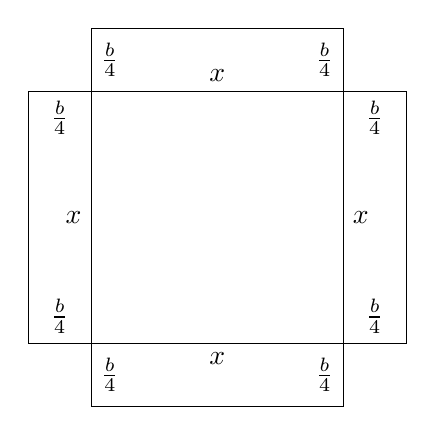
\begin{tikzpicture}[scale=.8]
\coordinate (A) at (0,0);
\coordinate (B) at (4,0);
\coordinate (C) at (4,4);
\coordinate (D) at (0,4);
\draw (A) -- node[below] {$x$} (B) -- node[right] {$x$} (C) -- node[above] {$x$} (D) -- node[left] {$x$} cycle;
\draw (A) -- node[right] {$\frac{b}{4}$} ++(0,-1) -- ++(4,0) -- node[left] {$\frac{b}{4}$} ++(0,1);
\draw (B) -- node[above] {$\frac{b}{4}$} ++(1,0) -- ++(0,4) -- node[below] {$\frac{b}{4}$} ++(-1,0);
\draw (C) -- node[left] {$\frac{b}{4}$} ++(0,1) -- ++(-4,0) -- node[right] {$\frac{b}{4}$} ++(0,-1);
\draw (D) -- node[below] {$\frac{b}{4}$} ++(-1,0) -- ++(0,-4) -- node[above] {$\frac{b}{4}$} ++(1,0);
\end{tikzpicture}
\caption{El área es $x^2+4(b/4)x=x^2+bx$}\label{f.khw-1}
\end{center}
\end{minipage}
\hfill
\begin{minipage}{.45\textwidth}
\begin{center}
\begin{tikzpicture}[scale=.8]
\coordinate (A) at (0,0);
\coordinate (B) at (4,0);
\coordinate (C) at (4,4);
\coordinate (D) at (0,4);
\draw (A) -- node[below] {$x$} (B) -- node[right] {$x$} (C) -- node[above] {$x$} (D) -- node[left] {$x$} cycle;
\draw (A) -- node[right] {$\frac{b}{4}$} ++(0,-1) -- ++(4,0) -- node[left] {$\frac{b}{4}$} ++(0,1);
\draw (B) -- node[above] {$\frac{b}{4}$} ++(1,0) -- ++(0,4) -- node[below] {$\frac{b}{4}$} ++(-1,0);
\draw (C) -- node[left] {$\frac{b}{4}$} ++(0,1) -- ++(-4,0) -- node[right] {$\frac{b}{4}$} ++(0,-1);
\draw (D) -- node[below] {$\frac{b}{4}$} ++(-1,0) -- ++(0,-4) -- node[above] {$\frac{b}{4}$} ++(1,0);
\draw[thick,dashed] ($(A)+(0,-1)$) -- ++(-1,0) -- ++(0,1);
\draw[thick,dashed] ($(B)+(0,-1)$) -- ++(1,0) -- ++(0,1);
\draw[thick,dashed] ($(C)+(0,1)$) -- ++(1,0) -- ++(0,-1);
\draw[thick,dashed] ($(D)+(0,1)$) -- ++(-1,0) -- ++(0,-1);
\end{tikzpicture}
\caption{El área es $x^2+4(b/4)x+4(b/4)^2=x^2+bx+(b^2/4)$}\label{f.khw-2}
\end{center}
\end{minipage}
\end{figure}

No podemos construir el diagrama en la figura~\ref{f.khw-1} porque no sabemos lo que $x$ es, pero el área del cuadrado más grande en la figura~\ref{f.khw-2} es:
\[
x^2+bx+\frac{b^2}{4}=c+\frac{b^2}{4}\,,
\]
que sí conocemos ya que los coeficientes $b,c$ son dados. Construyendo el diagrama y borrando los cuadraditos cuyos lados son $(b/4)$--otra cantidad conocida--obtenemos el segmento de longitud $x$.

\begin{example}
Sea $x^2+12x=64$. Entonces $c+(b^2/4)=64+36=100$. Es fácil construir un cuadrado de área $100$ ya que cada lado tiene longitud $10$. Ahora restamos $(b/4)+(b/4)=6$, los lados de los cuadrados más pequeños, para obtener $x=10-6=4$.
\end{example}

\section{Construcción de Cardano para resolver ecuaciones cúbicas}\label{s.cardano}

La fórmula para las raíces de las ecuaciones cúbicas fue publicada por primera vez en el siglo XVI por Gerolamo Cardano. No desarrollaremos aquí la fórmula, pero es interesante que la idea central se basa en una construcción geométrica similar a la de al-Khwarizmi. La construcción se puede obtener de forma muy sencilla utilizando el álgebra. Por multiplicación:
\begin{align}\label{eq.car}
(a+b)^3=a^3+3a^2b+3ab^2+b^3=(a^3+b^3)+3ab(a+b)\,.
\end{align}
Geométricamente, partimos de un cubo cuyo lado es $a+b$ de modo que su volumen es $(a+b)^3$. El cubo se descompone en cinco piezas. Las dos primeros son cubos cuyas caras son $a$ y $b$ con volúmenes $a^3$ (azul) y $b^3$ (rojo), respectivamente (Fig.~\ref{f.cardano1}).

Las otras tres partes son cajas (el término técnico es \emph{cuboide}) cada una con un lado de longitud $a+b$ que coincide con un lado del cubo, un lado de longitud $a$ y un lado de longitud $b$, de modo que el volumen de cada una de las tres cajas es $ab(a+b)$. En la figura~\ref{f.cardano2}, hay una caja en el lado izquierdo del cubo (azul), una en la parte posterior del cubo (rojo) y una en la parte superior del cubo (verde).
Combinando los cinco sólidos de la figura~\ref{f.cardano1} y la figura~\ref{f.cardano2} obtenemos la Ecuación~\ref{eq.car}.

\begin{figure}[tb]
\begin{center}
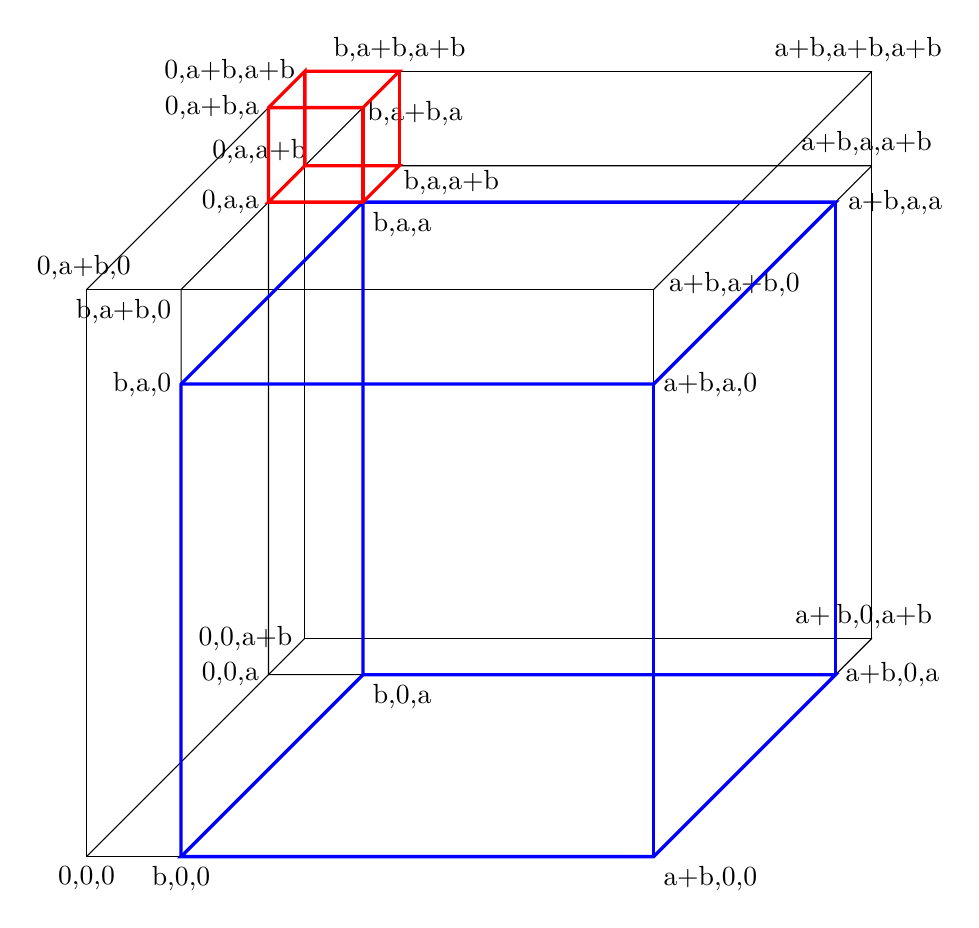
\begin{tikzpicture}[scale=1.2]

% Front face
\coordinate (A) at (0,0,0);
\node[below] at (A) {\sm{0,0,0}};
\coordinate (B) at (6,0,0);
\node[below right] at (B) {\sm{a+b,0,0}};
\coordinate (C) at (6,6,0);
\node[above right,xshift=2pt,yshift=-6pt] at (C)
  {\sm{a+b,a+b,0}};
\coordinate (D) at (0,6,0);
\node[above,xshift=-1pt] at (D) {\sm{0,a+b,0}};

% Front face
\coordinate (FF1) at (1,0,0);
\node[below] at (FF1) {\sm{b,0,0}};
\coordinate (FF2) at (1,5,0);
\node[left] at (FF2) {\sm{b,a,0}};
\coordinate (FF3) at (1,6,0);
\node[below left] at (FF3) {\sm{b,a+b,0}};
\coordinate (FF4) at (6,5,0);
\node[right] at (FF4) {\sm{a+b,a,0}};

% Back face
\coordinate (A1) at (0,0,-6);
\node[left,xshift=-1pt] at (A1) {\sm{0,0,a+b}};
\coordinate (B1) at (6,0,-6);
\node[above,xshift=-3pt] at (B1) {\sm{a+\:b,0,a+b}};
\coordinate (C1) at (6,6,-6);
\node[above,xshift=-5pt] at (C1) {\sm{a+b,a+b,a+b}};
\coordinate (D1) at (0,6,-6);
\node[left] at (D1) {\sm{0,a+b,a+b}};

% Back face
\coordinate (BF1) at (0,5,-6);
\node[above left,xshift=4pt,yshift=-3pt] at (BF1) 
  {\sm{0,a,a+b}};
\coordinate (BF2) at (1,5,-6);
\node[below right,xshift=-2pt,yshift=2pt] at (BF2)
  {\sm{b,a,a+b}};
\coordinate (BF3) at (1,6,-6);
\node[above] at (BF3) {\sm{b,a+b,a+b}};
\coordinate (BF4) at (6,5,-6);
\node[above,xshift=-2pt] at (BF4) {\sm{a+b,a,a+b}};

% Right face
\coordinate (RF1) at (6,5,-5);
\node[right,xshift=1pt] at (RF1) {\sm{a+b,a,a}};
\coordinate (RF2) at (6,0,-5);
\node[right] at (RF2) {\sm{a+b,0,a}};

% Bottom face
\coordinate (BT1) at (1,0,-5);
\node[below right] at (BT1) {\sm{b,0,a}};

% Left face
\coordinate (LF1) at (0,0,-5);
\node[left] at (LF1) {\sm{0,0,a}};
\coordinate (LF2) at (0,5,-5);
\node[left] at (LF2) {\sm{0,a,a}};
\coordinate (LF3) at (0,6,-5);
\node[left] at (LF3) {\sm{0,a+b,a}};

% Top face
\coordinate (TF1) at (1,6,-5);
\node[right,xshift=-2pt,yshift=-2pt] at (TF1) {\sm{b,a+b,a}};

% Internal point
\coordinate (I) at (1,5,-5);
\node[below right] at (I) {\sm{b,a,a}};


\draw (A) -- (B) -- (C) -- (D) -- cycle;
\draw (A1) -- (B1) -- (C1) -- (D1) -- cycle;
\draw (A) -- (A1);
\draw (B) -- (B1);
\draw (C) -- (C1);
\draw (D) -- (D1);

\draw (FF1) -- (FF2) -- (FF3) -- (BF3);
\draw (BF2) -- (FF2) -- (FF4) -- (BF4);
\draw (FF1) -- (BT1) -- (TF1);
\draw (BF3) -- (BF2);
\draw (TF1) -- (LF3);
\draw (LF3) -- (LF1) -- (RF2) -- (RF1) -- (LF2) -- 
      (BF1) -- (BF4);

\draw[very thick,blue] (FF1) -- (B) -- (RF2) -- (BT1) -- cycle; 
\draw[very thick,blue] (FF1) -- (FF2) -- (I) -- (BT1);
\draw[very thick,blue] (I) -- (RF1) -- (FF4) -- (FF2);
\draw[very thick,blue] (FF4) -- (B);
\draw[very thick,blue] (RF1) -- (RF2);

\draw[very thick,red] (I) -- (LF2) -- (BF1) -- (BF2) -- cycle;
\draw[very thick,red] (LF2) -- (LF3) -- (D1) -- (BF1);
\draw[very thick,red] (D1) -- (BF3) -- (TF1) -- (LF3);
\draw[very thick,red] (TF1) -- (I);
\draw[very thick,red] (BF3) -- (BF2);

\end{tikzpicture}
\end{center}
\caption{$(a+b)^3 = (a^3+b^3) + \cdots$}\label{f.cardano1}
\end{figure}

%%%%%%%%%%%%%%%%%%%%%%%%%%%%%%%%%%%%%%%%%%%%%%%%%%%%%%%%%%%%%

\begin{figure}[tb]
\begin{center}
\begin{tikzpicture}[scale=1.2]

% Front face
\coordinate (A) at (0,0,0);
\node[below] at (A) {\sm{0,0,0}};
\coordinate (B) at (6,0,0);
\node[below right] at (B) {\sm{a+b,0,0}};
\coordinate (C) at (6,6,0);
\node[above right,xshift=2pt,yshift=-6pt] at (C)
  {\sm{a+b,a+b,0}};
\coordinate (D) at (0,6,0);
\node[above,xshift=-1pt] at (D) {\sm{0,a+b,0}};

% Front face
\coordinate (FF1) at (1,0,0);
\node[below] at (FF1) {\sm{b,0,0}};
\coordinate (FF2) at (1,5,0);
\node[left] at (FF2) {\sm{b,a,0}};
\coordinate (FF3) at (1,6,0);
\node[below left] at (FF3) {\sm{b,a+b,0}};
\coordinate (FF4) at (6,5,0);
\node[right] at (FF4) {\sm{a+b,a,0}};

% Back face
\coordinate (A1) at (0,0,-6);
\node[left,xshift=-1pt] at (A1) {\sm{0,0,a+b}};
\coordinate (B1) at (6,0,-6);
\node[above,xshift=-3pt] at (B1) {\sm{a+\:b,0,a+b}};
\coordinate (C1) at (6,6,-6);
\node[above,xshift=-5pt] at (C1) {\sm{a+b,a+b,a+b}};
\coordinate (D1) at (0,6,-6);
\node[left] at (D1) {\sm{0,a+b,a+b}};

% Back face
\coordinate (BF1) at (0,5,-6);
\node[above left,xshift=4pt,yshift=-3pt] at (BF1) 
  {\sm{0,a,a+b}};
\coordinate (BF2) at (1,5,-6);
\node[below right,xshift=-2pt,yshift=2pt] at (BF2)
  {\sm{b,a,a+b}};
\coordinate (BF3) at (1,6,-6);
\node[above] at (BF3) {\sm{b,a+b,a+b}};
\coordinate (BF4) at (6,5,-6);
\node[above,xshift=-2pt] at (BF4) {\sm{a+b,a,a+b}};

% Right face
\coordinate (RF1) at (6,5,-5);
\node[right,xshift=1pt] at (RF1) {\sm{a+b,a,a}};
\coordinate (RF2) at (6,0,-5);
\node[right] at (RF2) {\sm{a+b,0,a}};

% Bottom face
\coordinate (BT1) at (1,0,-5);
\node[below right] at (BT1) {\sm{b,0,a}};

% Left face
\coordinate (LF1) at (0,0,-5);
\node[left] at (LF1) {\sm{0,0,a}};
\coordinate (LF2) at (0,5,-5);
\node[left] at (LF2) {\sm{0,a,a}};
\coordinate (LF3) at (0,6,-5);
\node[left] at (LF3) {\sm{0,a+b,a}};

% Top face
\coordinate (TF1) at (1,6,-5);
\node[right,xshift=-2pt,yshift=-2pt] at (TF1) {\sm{b,a+b,a}};

% Internal point
\coordinate (I) at (1,5,-5);
\node[below right] at (I) {\sm{b,a,a}};


\draw (A) -- (B) -- (C) -- (D) -- cycle;
\draw (A1) -- (B1) -- (C1) -- (D1) -- cycle;
\draw (A) -- (A1);
\draw (B) -- (B1);
\draw (C) -- (C1);
\draw (D) -- (D1);

\draw (FF1) -- (FF2) -- (FF3) -- (BF3);
\draw (BF2) -- (FF2) -- (FF4) -- (BF4);
\draw (FF1) -- (BT1) -- (TF1);
\draw (BF3) -- (BF2);
\draw (TF1) -- (LF3);
\draw (LF3) -- (LF1) -- (RF2) -- (RF1) -- (LF2) -- 
      (BF1) -- (BF4);

\draw[very thick,blue] (A) -- (FF1) -- (FF3) -- (D) -- cycle;
\draw[very thick,blue] (FF1) -- (BT1) -- (TF1) -- (FF3);
\draw[very thick,blue] (TF1) -- (LF3) -- (D);
\draw[very thick,blue] (LF3) -- (LF1) -- (A);
\draw[very thick,blue] (LF1) -- (BT1);

\draw[very thick,red] (LF1) -- (RF2) -- (RF1) -- (LF2);
\draw[very thick,red] ($(LF2) + (2pt,0)$) -- ($(LF1) + (2pt,0)$);
\draw[very thick,red] (A1) -- (B1) -- (BF4) -- (BF1) -- cycle;
\draw[very thick,red] ($(LF2) + (2pt,0)$) -- ($(BF1) + (2pt,0)$);
\draw[very thick,red] (BF4) -- (RF1);
\draw[very thick,red] (B1) -- (RF2);
\draw[very thick,red] (A1) -- (LF1);

\draw[very thick,green] (FF2) -- (FF4) -- (C) -- (FF3);
\draw[very thick,green] 
  ($(FF2) + (2pt,0)$) -- ($(FF3) + (2pt,0)$);
\draw[very thick,green] 
  ($(FF4) + (0,2pt)$) -- ($(BF4) + (0,2pt)$);
\draw[very thick,green] (BF4) -- (C1) -- (BF3);
\draw[very thick,green] 
  ($(BF3) + (2pt,0)$) -- ($(FF3) + (2pt,0)$);
\draw[very thick,green] (C1) -- (C);
\draw[very thick,green] (BF3) -- (BF2) -- (FF2);
\draw[very thick,green] 
  ($(BF2) + (0,2pt)$) -- ($(BF4) + (0,2pt)$);


\end{tikzpicture}
\end{center}
\caption{$(a+b)^3 = \cdots + 3ab(a+b)$}\label{f.cardano2}
\end{figure}

\section{No los intimidaban los números imaginarios}\label{s.imaginary}

La historia de las matemáticas muestra una progresión de conceptos que inicialmente se consideraron sin sentido, pero que finalmente se comprendieron, aceptaron y demostraron su utilidad. <<Obviamente,>> como los números enumeran (cuentan) objetos, $-1$, un número negativo, no tiene sentido. <<Obviamente,>> puesto que los números son cocientes de números enteros (números racionales), $\sqrt{2}$, que puede demostrarse fácilmente que es irracional, no tiene sentido. <<Obviamente,>> $\sqrt{-1}$, la raíz cuadrada de un número negativo, no tiene sentido, ya que no hay ningún número --entero, racional o real-- cuyo cuadrado sea $-1$.

La comprensión completa de las raíces cuadradas de los números negativos, hasta hoy llamados \emph{números imaginarios} aunque no son menos reales que los números reales, no se alcanzó hasta el siglo XIX. Por eso sorprende que, ya en el siglo XVI, Geralamo Cardano y Rafael Bombelli se negaran a dejarse intimidar por el concepto y dieran los primeros pequeños pasos hacia la comprensión de estos números.

Consideremos la ecuación cuadrática:
\begin{align}
x^2-10x+40=0\,.\label{eq.cardano-quadratic}
\end{align}
Según la conocida fórmula (Ecuación~\ref{eq.quadratic-roots}):
\[
r_1, r_2=\displaystyle\frac{10\pm\sqrt{100-160}}{2}=5\pm\sqrt{-15}\,.
\]
Bueno, no sabemos nada acerca de las raíces cuadradas de los números negativos y no sabemos cuáles son estos valores, pero como Cardano sabemos por el Teorema~\ref{eq.quadratic-roots} que:
\[
\begin{array}{lcl}
r_1+r_2&=&(5+\sqrt{-15})+(5-\sqrt{-15})=10=-b\\
r_1r_2&=&(5+\sqrt{-15})(5-\sqrt{-15})=25-5\sqrt{-15}+5\sqrt{-15}-(-15)=40=c\,.
\end{array}
\]
que se corresponden con los coeficientes de la ecuación cuadrática (Ecuación~\ref{eq.cardano-quadratic}). Es bastante intuitivo que $\sqrt{-15}+(-\sqrt{-15})=0$ aunque no sepamos nada de $\sqrt{-15}$, y, del mismo modo, es bastante intuitivo que $\sqrt{-15}\cdot-(\sqrt{-15})=-(-15)=15$ aunque no sepamos qué es $\sqrt{-15}$.

Consideremos ahora la ecuación cúbica:
\begin{align}
x^3-15x-4=0\,.\label{eq.bombelli-cubic}
\end{align}
No es difícil observar que $4$ es una raíz, pero ¿cómo se puede calcular? La fórmula de Cardano da la raíz:
\begin{align}
r=\sqrt[3]{2+11\sqrt{-1}}+\sqrt[3]{2-11\sqrt{-1}}\,,\label{eq.cube-root}
\end{align}
una fórmula bastante complicada que no tiene ninguna relación evidente con $4$. 

Bombelli realizó valientemente el siguiente cálculo (véase la Ecuación.~\ref{eq.car}):
\begin{eqnarray*}
(2+\sqrt{-1})^3&=&
8+3\cdot 4\sqrt{-1}+3\cdot 2(-1)+(-1\sqrt{-1})=
2+11\sqrt{-1}\\
(2-\sqrt{-1})^3&=&
8-3\cdot 4\sqrt{-1}+3\cdot 2(-1)-(-1\sqrt{-1})=
2-11\sqrt{-1}\,,
\end{eqnarray*}
y por la Ecuación~\ref{eq.cube-root}:
\begin{eqnarray*}
r&=&\sqrt[3]{2+11\sqrt{-1}} + \sqrt[3]{2-11\sqrt{-1}}\\
&=&\sqrt[3]{(2+\sqrt{-1})^3} + \sqrt[3]{(2-\sqrt{-1})^3}\\
&=&(2+\sqrt{-1}) + (2-\sqrt{-1})=4\,.
\end{eqnarray*}

%%%%%%%%%%%%%%%%%%%%%%%%%%%%%%%%%%%%%%%%%%%%%%%%%%%%%%%%

\section{El método de Lill y el círculo de Carlyle}\label{s.lill-quadratic}

El método de Lill se puede aplicar para resolver ecuaciones cuadráticas\footnote{Esta sección asume que has leído sobre el método de Lill en el Capitulo~\ref{c.origami-cube}.}. Como ejemplo usamos la Ecuación~\ref{eq.quadratic-lill} que da las raíces de una ecuación cuadrática obtenidas por factorización:
\[
x^2+bx+c=x^2-4x+3= (x-1)(x-3)\,.
\]
Aplicando el método de Lill se obtienen las trayectorias mostradas en la figura~\ref{f.lill-quadratic}.

\begin{figure}[bt]
\begin{center}
\begin{tikzpicture}[scale=1.1]
% Draw help lines and axes
\draw[step=10mm,white!50!black] (-4,-5) grid (2,1);
\draw[thick] (-4,0) -- (2,0);
\draw[thick] (0,-5) -- (0,1);
\foreach \x in {-3,...,2}
  \node at (\x-.2,.2) {\sm{\x}};
\foreach \y in {-4,...,-1}
  \node at (-.2,\y-.3) {\sm{\y}};

 Draw first path
\coordinate (A) at (0,0);
\coordinate (B) at (1,0);
\coordinate (C) at (1,-4);
\coordinate (D) at (-2,-4);
\draw[very thick] (A) --
  node[above] {$1$} (B);
\draw[very thick,name path=bc] (B) -- 
  node[right,xshift=-1pt,yshift=6pt] {$b=-4$} (C);
\draw[very thick,name path=cd] (C) --
  node[below left,xshift=3pt] {$c=3$}(D);

% Draw first segment of second path
\path[name path=a2] (A) -- +(-45:1.414);
\path [name intersections = {of = a2 and bc, by = {A2}}];
\node[above right] at (A2) {$P_1$};
\draw[very thick,dashed] (A) -- (A2);
\draw ($(A) + (14pt,0)$)
  arc [start angle=0, end angle = -45, radius=14pt];
\node[below right,xshift=40pt,yshift=-2pt] at (A) {$-45^\circ$};
\draw[->] ($(A)+(33pt,-6pt)$) -- +(-18pt,0);
\draw[rotate=135] (A2) rectangle +(5pt,5pt);

% Draw second segment of second path
\path[name path=b2] (A2) -- +(-135:5);
\path [name intersections = {of = b2 and cd, by = {B2}}];
\draw[very thick,dashed] (A2) -- (B2);

% Draw first segment of second path
\path[name path=a3] (A) -- +(-71.57:4);
\path [name intersections = {of = a3 and bc, by = {A3}}];
\node[above right] at (A3) {$P_2$};
\draw[very thick,dashed] (A) -- (A3);
\draw ($(A) + (20pt,0)$)
  arc [start angle=0, end angle = -71.57, radius=20pt];
\node[below right,xshift=40pt,yshift=-10pt] at (A) {$-71.57^\circ$};
\draw[->] ($(A)+(35pt,-13pt)$) -- +(-18pt,0);
\draw[rotate=108.43] (A3) rectangle +(5pt,5pt);

% Draw second segment of second path
\path[name path=b3] (A3) -- +(198.43:5);
\path [name intersections = {of = b3 and cd, by = {B3}}];
\draw[very thick,dashed] (A3) -- (B3);

\end{tikzpicture}
\end{center}
\caption{Método de Lill en $x^2-4x+3$}\label{f.lill-quadratic}
\end{figure}
Comprobamos que los ángulos son correctos:
\[
-\tan (-45^\circ) = -1,\quad -\tan (-71.57^\circ) \approx -3\,.
\]
Para las ecuaciones cuadráticas podemos encontrar los puntos $P_1,P_2$ como las intersecciones de la recta que representa el coeficiente $b$ y el círculo cuyo diámetro es la recta que une el punto inicial y el punto final de las trayectorias (Fig.~\ref{f.lill-circle}). Para que un punto de la recta $b$ sea una raíz, la reflexión de la recta debe ser $90^\circ$ y, por tanto, el ángulo inscrito es subtendido por un diámetro.

\begin{figure}[t]
\begin{center}
\begin{tikzpicture}[scale=1]
% Draw help lines and axes
\draw[step=10mm,white!50!black] (-4,-5) grid (2,1);
\draw[thick] (-4,0) -- (2,0);
\draw[thick] (0,-5) -- (0,1);
\foreach \x in {-3,...,2}
  \node at (\x-.2,.2) {\sm{\x}};
\foreach \y in {-4,...,-1}
  \node at (-.2,\y-.3) {\sm{\y}};

 Draw first path
\coordinate (A) at (0,0);
\coordinate (B) at (1,0);
\coordinate (C) at (1,-4);
\coordinate (D) at (-2,-4);
\draw[very thick] (A) --
  node[above] {$1$} (B);
\draw[very thick,name path=bc] (B) -- 
  node[right,xshift=-2pt,yshift=6pt] {$b=-4$} (C);
\draw[very thick,name path=cd] (C) --
  node[below left,xshift=-1pt,yshift=-5pt] {$c=3$}(D);

% Draw first segment of second path
\path[name path=a2] (A) -- +(-45:1.414);
\path [name intersections = {of = a2 and bc, by = {A2}}];
\node[above right] at (A2) {$P_1$};
\draw[dashed] (A) -- (A2);
\draw ($(A) + (14pt,0)$)
  arc [start angle=0, end angle = -45, radius=14pt];
\node[below right,xshift=40pt,yshift=-2pt] at (A) {$-45^\circ$};
\draw[->] ($(A)+(33pt,-6pt)$) -- +(-18pt,0);
\draw[rotate=135] (A2) rectangle +(5pt,5pt);

% Draw second segment of second path
\path[name path=b2] (A2) -- +(-135:5);
\path [name intersections = {of = b2 and cd, by = {B2}}];
\draw[dashed] (A2) -- (B2);

% Draw first segment of second path
\path[name path=a3] (A) -- +(-71.57:4);
\path [name intersections = {of = a3 and bc, by = {A3}}];
\node[above right] at (A3) {$P_2$};
\draw[dashed] (A) -- (A3);
\draw ($(A) + (20pt,0)$)
  arc [start angle=0, end angle = -71.57, radius=20pt];
\node[below right,xshift=40pt,yshift=-10pt] at (A) {$-71.57^\circ$};
\draw[->] ($(A)+(35pt,-13pt)$) -- +(-18pt,0);
\draw[rotate=108.43] (A3) rectangle +(5pt,5pt);

% Draw second segment of second path
\path[name path=b3] (A3) -- +(198.43:5);
\path [name intersections = {of = b3 and cd, by = {B3}}];
\draw[dashed] (A3) -- (B3);

\coordinate (O) at (-1,-2);
\vertex{O};
\node[draw,circle through=(A)] at (O) {};
\draw[very thick,dotted] (A) -- (D);

\end{tikzpicture}
\end{center}
\caption{Construimos un círculo para encontrar las raíces}\label{f.lill-circle}
\end{figure}

Esto también se puede comprobar por cálculo. El centro del círculo es el punto medio del diámetro $(-1,-2)$. La longitud del diámetro es:
\[
\sqrt{(-2)^2+(-4)^2}=\sqrt{20}\,,
\]
por lo que el cuadrado de la longitud del radio es $\left(\sqrt{20/2}\right)^2=5$. Necesitamos la intersección de esta circunferencia con la recta $x=1$:
\begin{eqnarray*}
(x-(-1))^2+(y-(-2))^2&=&r^2\\
(x^2+2x+1)+(y^2+4y+4)&=&5\\
y^2+4y+3&=&0\\
y&=&-1,\;-3\,.
\end{eqnarray*}
Un método similar para resolver ecuaciones cuadráticas es el círculo de Carlyle, que es anterior al método de Lill. Dada una ecuación cuadrática $x^2-bx+c$ (nótese el signo menos en el término lineal), construimos puntos en $(0,1)$ y $(b,c)$. Construimos una circunferencia cuyo diámetro sea la recta que une los dos puntos (Fig.~\ref{f.carlyle-circle}). Sus intersecciones (si las hay) con el eje $x$ son las raíces de la ecuación.

En el caso general, el centro del círculo es $(b/2,(c-(-1))/2)$ y la longitud del diámetro es $\sqrt{b^2+(c-1)^2}$, por lo que la ecuación del círculo es:
\[
\left(x-\frac{b}{2}\right)^2+\left(y-\frac{c+1}{2}\right)^2=
\frac{b^2+(c-1)^2}{4}\,.
\]
Para el ejemplo, sustituyendo $b=4,c=3$ y $y=0$, vemos que $x=1$ y $x=3$ son las raíces de la ecuación cuadrática.

\begin{figure}[t]
\begin{center}
\begin{tikzpicture}[scale=1]
% Draw help lines and axes
\draw[step=10mm,white!50!black] (-1,-1) grid (5,5);
\draw[thick] (-1,0) -- (5,0);
\draw[thick] (0,-1) -- (0,5);
\foreach \x in {0,...,5}
  \node at (\x-.2,.2) {\sm{\x}};
\foreach \y in {1,...,4}
  \node at (-.1,\y+.2) {\sm{\y}};

\coordinate (A) at (0,1);
\node[below left] at (A) {$(0,1)$};
\coordinate (B) at (4,3);
\node[above right] at (B) {$(4,3)$};
\vertex{A};
\vertex{B};

\coordinate (O) at (2,2);
\vertex{O};
\node[draw,circle through=(B)] at (O) {};
\draw[very thick,dotted] (A) -- (B);

\coordinate (X1) at (1,0);
\node[below left] at (X1) {$(1,0)$};
\coordinate (X2) at (3,0);
\node[below right] at (X2) {$(3,0)$};
\vertex{X1};
\vertex{X2};

\end{tikzpicture}
\end{center}
\caption{Círculo Carlyle para $x^2-4x+3$}\label{f.carlyle-circle}
\end{figure}


\section{Cálculo numérico de las raíces}\label{s.numerical}
\index{Quadratic equation!numerical computation of the roots}

Los alumnos aprenden cálculo simbólico de raíces, derivadas, etc. Hoy en día, la mayoría de los cálculos se realizan por ordenador, por lo que el cálculo simbólico es menos importante. El \emph{análisis numérico} es la rama de las matemáticas y la informática que desarrolla métodos de cálculo precisos y eficaces. El principal reto es hacer frente a la finitud de los valores almacenados en la memoria del ordenador. El cálculo:
\[0.12 \times 0.14=0.0168\]
es fácil de hacer, pero:
\[
0.123456789\times 0.123456789\]
necesita dieciocho dígitos para ser representado con precisión y esto no puede hacerse con una memoria que almacena dieciséis dígitos. El cálculo incurrirá en un error de redondeo.

Un problema aún más grave se encuentra cuando se realiza \emph{aritmética de punto flotante}. Claramente:
\[(0.12\times 10^{-10})\times (0.14\times 10^{-8})\]
no se calcularía escribiendo todos los dígitos que son cero. En su lugar, multiplicamos las mantisas y sumamos los exponentes para obtener $0,0168\times 10^{-18}$, que se normaliza a $0,168\times 10^{-19}$ para que el dígito más significativo aparezca después del punto decimal, asegurando la máxima precisión dado el tamaño fijo de la mantisa. Si el exponente máximo que se puede representar es $-16$ el resultado simplemente no se puede almacenar. Este error se denomina desbordamiento de punto flotante.

La fórmula para encontrar las raíces de la ecuación cuadrática $x^2+bx+c$ es:
\begin{align}
r_1, r_2 = \frac{-b\pm\sqrt{b^2-4c}}{2}\,.\label{eq.quadratic-numerical}
\end{align}
Consideremos que ocurre si $b=1000$ and $c=4$. Las raíces son:
\[
r_1, r_2 = \frac{-1000\pm\sqrt{1000000-16}}{2}\,.
\]
Dependiendo de la precisión de la aritmética, es posible que una de las raíces esté tan cerca de cero que el valor almacenado sea cero. Evaluamos la ecuación cuadrática da el sorprendente resultado $0^2+b\cdot 0 +4= 4= 0$.

¿Podemos hacerlo mejor? Por la Ecuación~\ref{eq.viete-quad}:
\[
r_1+r_2 = -b\,,\quad\quad r_1r_2=c\,.
\]
Si $r_2$ es mucho menor que $r_1$, que se denota $r_2\ll r_1$, entonces $r_1\approx -b$ y $r_2\approx c/b$. En la tabla~\ref{t.quadratic}, calculada por un programa informático, se comparan los valores de las raíces calculadas por estas fórmulas con los valores obtenidos de la fórmula tradicional (Ecuación~\ref{eq.quadratic-numerical}). El valor de $c$ se fija en $4$ y se muestran las raíces para valores crecientes de $b$.

Inicialmente, los valores reales calculados mediante la fórmula tradicional para $r_2$ son más exactos ($r_2-r_{2v}$ es negativo), pero a partir de $b=100000$, el cálculo basado en la Ecuación~\ref{eq.viete-quad} es más exacto. Tales son las sorpresas del análisis numérico.

\begin{table}[bht]
\caption[Dos cálculos de las raíces de una ecuación cuadrática]{Dos cálculos de las raíces de una ecuación cuadrática. $r_1,r_2$ son las raíces calculadas por la Ecuación~\ref{eq.quadratic-numerical}. $r_{1v},r_{2v}$ son las raíces calculadas mediante la Ecuación~\ref{eq.viete-quad}. Los errores son $r_{i}-r_{iv}$. Los valores se truncan a cuatro decimales.
Los números en coma flotante se escriben $-4e-5$ en lugar de $4\times 10^{-5}$ porque los programas de ordenador se escriben normalmente como secuencias lineales de caracteres.} \label{t.quadratic}

\begin{scriptsize}
\[
\begin{array}{r@{\hspace{2.5mm}}r@{\hspace{2.5mm}}r@{\hspace{2.5mm}}r@{\hspace{2.5mm}}r@{\hspace{2.5mm}}r@{\hspace{2.5mm}}r}
\hline
\noalign{\smallskip}
b & r_1 & r_{1v} & \mathrm{Error}_1 & r_2 & r_{2v} & \mathrm{Error}_2\\
\noalign{\smallskip}\hline\noalign{\smallskip}
100  &  -99.9599  &  -100  &  0.0400  &  -0.04001\  &  -0.04  &  -1.6012e\!-\!05\\
1000  &  -999.9959  &  -1000  &  0.0040  &  -0.0040  &  -0.004  &  -1.6000e\!-\!08\\
10000  &  -9999.9996  &  -10000  &  0.0004  &  -0.0004  &  -0.0004  &  -1.6270e\!-\!11\\
100000  &  -99999.9999  &  -100000  &  3.9999e\!-\!5  &  -3.9999e\!-\!5  &  -4e\!-\!5  &  1.0104e\!-\!12\\
1000000  &  -999999.9999  &  -1000000  &  4.0000e\!-\!6  &  -3.9999e\!-\!6  &  -4e\!-\!6  &  2.7749e\!-\!11\\
10000000  &  -10000000.0  &  -10000000  &  3.9860e\!-\!7  &  -3.9953e\!-\!7  &  -4e\!-\!7  &  4.6261e\!-\!10\\
 \noalign{\smallskip}
 \hline
\end{array}
\]
\end{scriptsize}
\end{table}

\subsection*{¿Cuál es la sorpresa?}

El enfoque de Poh-Shen Loh proporciona una nueva forma de ver la relación entre los coeficientes y las raíces que no se ve simplemente memorizando la fórmula tradicional. Lo sorprendente es que esta relación es fundamental en la demostración algebraica de Gauss de la constructibilidad de un heptadecágono regular (Capítulo~\ref{c.heptadecagon}).

Con el dominio moderno de los métodos algebraicos en geometría, es importante recordar que antes ocurría lo contrario. Como lo demuestran las construcciones de Al-Khwarizmi y Cardano, los métodos geométricos se utilizaban para obtener resultados en álgebra. Lill y Carlyle desarrollaron métodos geométricos para resolver ecuaciones cuadráticas. Las consideraciones sobre el cálculo numérico en los ordenadores sorprenderán a los alumnos que no lo hayan experimentado antes.

\subsection*{Fuentes}

El método de Poh-Shen Loh procede de \cite{loh1,loh2}. La construcción de Al-Khwarizmi se encuentra en \cite[Capítulo~1]{jorg} y \cite{mastin}. La construcción de Cardano se encuentra en \cite[Capítulo~1]{jorg}. Para la colorida historia del desarrollo de la fórmula de Cardano, véase \cite{wiki:cardano}. Los primeros intentos de calcular con números imaginarios están en \cite[Capítulo~2]{jorg}. El método de Lill y el círculo de Carlyle se pueden encontrar en \cite{wiki:quadratic} junto con una discusión del cálculo numérico de las raíces.
